\documentclass[a4paper,11pt]{article}

\usepackage[plain]{fullpage} 
\usepackage{graphicx}  
\usepackage{wrapfig}
\usepackage{float}
\usepackage{array}
\usepackage[hidelinks]{hyperref}
\usepackage{color}
\definecolor{light-gray}{gray}{0.95}
\usepackage{listings}
\lstset{
basicstyle=\scriptsize, 
morecomment=[l]{/*},
backgroundcolor=\color{light-gray}, 
xleftmargin=.10in,
xrightmargin=.10in,
language=C
}

\renewcommand{\arraystretch}{1.25} %vertical cell padding

\title{\textbf{Report: Assignment 3}}
\author{Group 9: \O yvin Richardsen, Sandor Zeestraten, Stian Habbestad}
\date{{Norwegian University of Science and Technology \\
TDT4258 Energy Efficient Computer Design \\}
\today}

\begin{document}
\maketitle

\begin{abstract}
In this assignment the goal is to program a simple computer game in C for an AVR32 micro controller running Linux. To accomplish this one needs to understand and write Linux device drivers for I/O. We therefore wrote our own drivers for operating LEDs and switches on the development board. The game we chose to implement is a simple puzzle game called Sokoban.
\end{abstract}

\bigskip
\tableofcontents
\newpage

\section{Introduction}
In this exercise we start out with installing Linux on the STK1000 development board from the SD card. We are now able to write C code that benefits from Linux functions. %Greit nok formulert?  
To be able to communicate with the LEDs and the buttons on the STK1000 development board we wrote a pair of drivers for Linux with great help from \textit{"Linux Device Drivers, Third Edition"} \cite{ldd}


\section{Description and methodology}
\textbf{Forrige rapport: organize report better (overview and block diagram before description of code fragments and functions). Ergo, block diagram her?}\\

%Nevne uboot og bootloader
First off we started out with trying to install Linux on the STK1000 development board. This turned out to be a tricky affair. We had a step by step guide for compiling Linux that we followed, but with no luck. Luckily there was mentioned an image of a precompiled Linux that we could extract to the SD card. After some mixing back and forth with environment variables from the other u-boot.bin file(from Itslearning) into the one we were using we finally started to get somewhere. Another group posted a guide on Itslearning that worked for us.

Once we had Linux up and running we started out with a simple "Hello world" program to verify that things were working. Now we started out with programming a driver for the LEDs. We sometimes thought we had found the solution, but we weren't quite right yet. We gave the LED driver a pause and started to communicate with the frame buffer in Linux instead. 

First off we thought maybe this file had to be a kernel module as well, but we soon understood that we needed access to quite a few libraries to make the memory mapping work. We started with generating a random bit values for the display and went on with more logical values, for example a third of the screen was made red. As we tried to read bit values from an image of the file format bitmap, we started to see that there were some errors in regards to how we read the file. After a lot of trial and error we finally managed to display the image files properly. We organized the screen into a grid of 20 by 15 tiles built up of 16 by 16 pixels for each tile. This made it easy to map the \textit{charmap} to the images and render the levels on the LCD screen. It is also a fairly convenient size for the game when it comes to the variety of the sizes of each level.

From the previous exercise we learned how to handle sound in C which came in handy for the game sounds. We wanted the player to get good feedback through sound effects by telling the player when he does something right or wrong. Therefore we constructed a negative sound when you hit the wall or removed a crate from a target and a more positive sound when you push a crate on a target. 

\subsection{The game}
\subsubsection{Sokoban}
The game we chose to implement was a simple top-down puzzle game called \textit{Sokoban}\cite{sokoban}. The point of the game is for the player to push boxes onto marked goal squares. The levels are small maps confined by walls which cannot be walked through. The puzzle is solved when all the boxes are on the goal squares. We had some previous experience of implementing this game in Java in the course TDT4100: Object Oriented Programming. We therefore chose to port it to C. See figure~\ref{fig:sokobanscreen} for a screenshot of a level in Sokoban.

\begin{figure}[H]
\centering
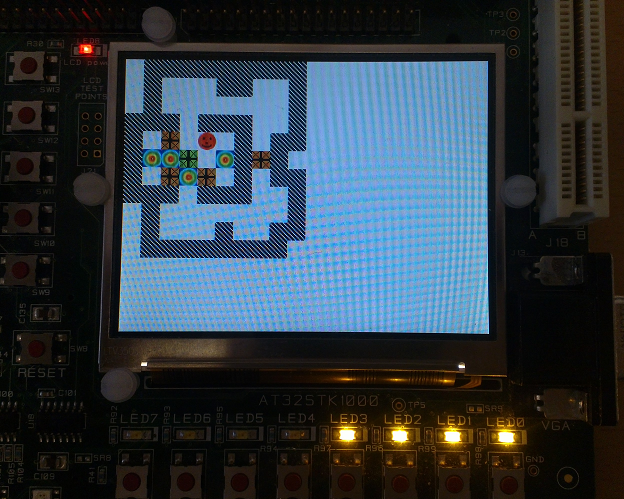
\includegraphics[scale=0.4]{images/sokobanscreen.png}
\caption{A screenshot of a level in Sokoban.}
\label{fig:sokobanscreen}
\end{figure}

\subsubsection{Levels}
The levels are defined by it's dimensions and an array of characters of the different elements. For more information see the level format page on Sokoban Wiki \cite{sokobanlevel}. The  table~\ref{tab:levelformat} shows the level format we used. For an example of how the levels are designed, see figure~\ref{fig:leveldef}. This level 1 and it is the simplest solvable level. The only move available is to push the box to the left. Figure~\ref{fig:level1} shows how it looks on the STK1000.

\begin{table}[H]
\centering
\begin{tabular}{|l|l|l|}
\hline \textbf{Level element} & \textbf{Character} & \textbf{Graphics} \\ 
\hline Wall & \# & 
\includegraphics[scale=0.6]{images/wall.png} \\ 
\hline Player & @ & 
\includegraphics[scale=0.6]{images/player.png} \\ 
\hline Player on goal square & + & 
\includegraphics[scale=0.6]{images/playertarget.png} \\ 
\hline Box & \$ & 
\includegraphics[scale=0.6]{images/crate.png}\\ 
\hline Box on goal square & * & 
\includegraphics[scale=0.6]{images/cratetarget.png}\\ 
\hline Goal square & . & 
\includegraphics[scale=0.6]{images/target.png}\\ 
\hline Floor & (whitespace) & 
\includegraphics[scale=0.6]{images/blank.png} \\ 
\hline 
\end{tabular}
\caption{The level format.}
\label{tab:levelformat}
\end{table}

\begin{figure}[H]
\begin{lstlisting}
// From sokoban_leveldefs.h
#define level1dimX 5
#define level1dimY 3
char level1[] = "######@$.######";
\end{lstlisting}
\caption{Definition of the level 1.}
\label{fig:leveldef}
\end{figure}

\begin{figure}[H]
\centering
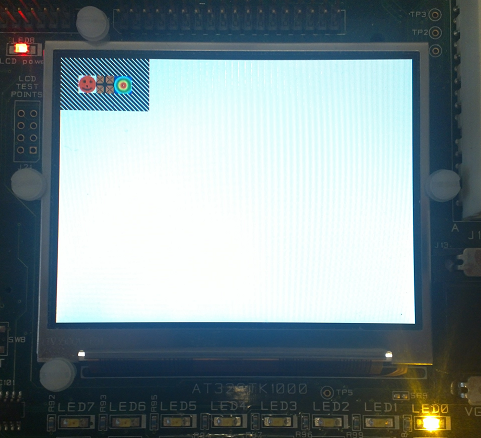
\includegraphics[scale=0.5]{images/level1.png}
\caption{Level 1 running on the STK1000.}
\label{fig:level1}
\end{figure}

\subsubsection{Game logic}

\subsection{Drivers}
In order to interact with the development board we wrote two separate device drivers. One for the LEDs and one for the buttons. 
\subsubsection{LEDs}

\subsubsection{Buttons}

\subsection{Debugging}
\begin{figure}[H]
\centering
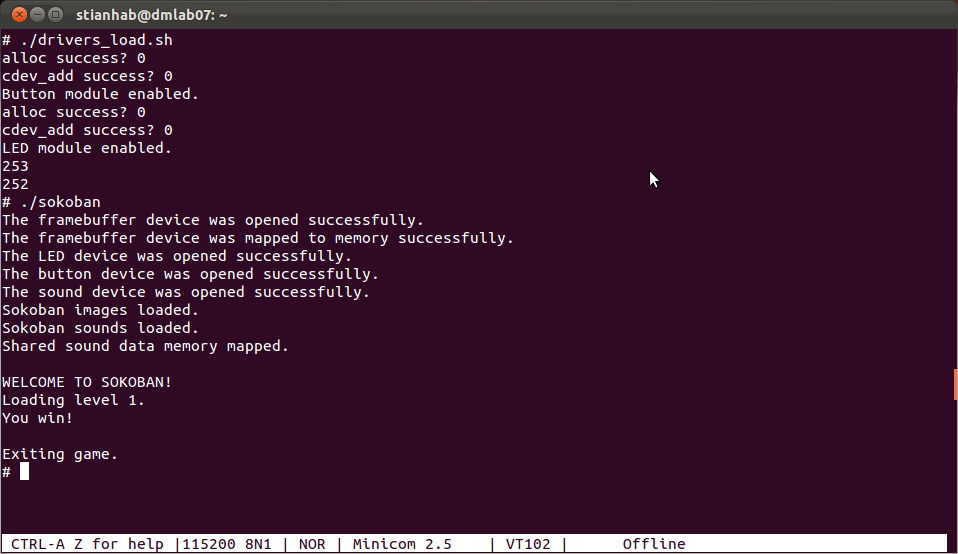
\includegraphics[scale=0.4]{images/consolestart.png}
\caption{Loading of device drivers and running the game from the console.}
\label{fig:consolestart}
\end{figure}

%State diagrams

%Here is a screenshot (Figure 2) showing us debugging our \emph{generateTriangle} function which generates triangle sound wave samples. More specifically we check that the values we get from each part of our (complex) mathematical expression are valid. 

\section{How to setup, build and play}
\subsection{STK1000 setup}
Make sure that all the jumpers and cables are connected as described in section 4.3.3 in the TDT4258 Compendium \cite{komp}.
In addition, use the following setup for the GPIO, buttons and LEDs.

\begin{itemize}
\item Connect J1 to Switches
\item Connect J2 to Buttons
\end{itemize}

\subsection{Build instructions}
We've setup our build environment to automatically upload the necessary files to the development board. Should you want upload and run the compiled binaries yourself, then simply upload the files found in the \textit{bin} directory to the \textit{root} directory of the board and continue with the run instruction.

\paragraph{Drivers}
In the \textit{driver} directory, edit the \textit{compile\_and\_upload\_drivers.sh} script and set the correct IP address of the board. Then run the script which compiles and uploads them.

\paragraph{Game}
In the \textit{sokoban} directory, edit the \textit{Makefile} and again edit the IP of the board. Then run \textit{make} and \textit{make send}.

\subsection{Run instructions}
Connect to the board with \textit{Minicom} as described in the compendium. Run the \textit{drivers\_load.sh} script to load the drivers. Then to start the game, simply run the \textit{sokoban} executable. See figure~\ref{fig:consolestart} for the console output if the drivers and the game runs successfully. 

\section{Results}
\subsection{Description} 

This exercise resulted in a working Sokoban game on the STK1000 development board displayed. The game is played by using the buttons as controllers to move around in the game which is displayed on the LCD screen. In addition to a general "arrow key" setup, there is also a possibility to undo and redo with the buttons. For a quick view of how the game operates see our gameplay video on Youtube\cite{youtube}.

\subsection{Feedback}There are sounds and LEDs to help you understand the game play better through audiovisual feedback. The LEDs show how many crates you have left in the game, and when you win all LEDs will blink several times.

\subsection{Levels}
We 

\subsection{Sounds}There are sounds for the start of the game, when you place a crate on a target, when you remove a crate from a target, when you hit a wall and when you win. When you win there will also be a splash screen telling you that you've won. 

\subsection{Game play}
In regards to the game play we have movement in four directions, the ability to push crates, disability to walk through walls, and the ability to undo and redo. 

\subsection{Game controls}
The controls of the game are listed below in table~\ref{tab:gamecontrols}. 
\begin{table}[H]
\centering
\begin{tabular}{|l|l|}
\hline \textbf{Switch} & \textbf{Action} \\ 
\hline SW7 & Move left \\ 
\hline SW6 & Move down \\ 
\hline SW5 & Move up \\ 
\hline SW4 & Move right \\ 
\hline SW3 & Undo move \\ 
\hline SW2 & Redo move \\ 
\hline SW1 & Reset level \\ 
\hline SW0 & Main menu \\
\hline 
\end{tabular}
\caption{Game controls} 
\label{tab:gamecontrols}
\end{table}

\subsection{Technical aspects}Technically the resulting game is written in C code on top of a Linux operating system. To manage the LEDs and buttons we have written two corresponding Linux drivers that operates as interfaces between the STK1000 development board and Linux. 

\section{Tests}
\subsection{Description}

We've created a few test scenarios in order to test different aspects of our game functionality. The tests were conducted by a person interacting with the switches and looking at the LCD screen, wearing a headset. Another person logged the results of the test. The main equipment was the STK1000 development board and a headset with the main focus on the LCD screen. The jumpers of the board were set as specified in the compendium (section 4.2) \cite{komp}. The GPIO was set up with both LEDs and switches connected to B as follows: LEDs on 8-15, switches on 0-7. 

\subsection{Results}
Below is a table of the different tests we ran, the preconditions and the results. 

\begin{center}
\scriptsize
\renewcommand{\arraystretch}{1.25} %vertical cell padding
\begin{tabular}[pos]{|m{35pt}|m{45pt}|m{80pt}|m{90pt}|m{105pt}|m{40pt}|}
\hline \textbf{Number} & \textbf{Name} & \textbf{Description} & \textbf{Conditions} & \textbf{Expected} & \textbf{Results} \\ 

\hline 1 & Steady-state test & Power is on and the main program is running & The board has been programmed and powered on & The board is powered and no LEDs or sounds should be on & Passed \\

\hline 2 & Left & Player is moved left & A level is loaded and there is free space to the left of the player & Player moves to the left when \emph{SW7} is pressed.  & Passed \\

\hline 3 & Down & Player is moved down & A level is loaded and there is free space beneath the player & Player moves down when \emph{SW6} is pressed.  & Passed \\

\hline 4 & Up & Player is moved up & A level is loaded and there is free space above the player & Player moves up when \emph{SW5} is pressed.  & Passed \\

\hline 5 & Right & Player is moved right & A level is loaded and there is free space to the right of the player & Player moves to the right when \emph{SW4} is pressed.  & Passed \\

\hline 6 & Undo & The last move is undone & At least one move is made & The last move is undone when \emph{SW3} is pressed.  & Passed \\

\hline 7 & Redo & The last undo is undone & Undo must have been done as the previous move. & The undone move is redone when \emph{SW2} is pressed.  & Passed \\

\hline 8 &  Reset level & The loaded level is reset & A level must have been loaded and the game may or may not have been initialized & Level is reset when \emph{SW1} is pressed.  & Passed \\

\hline 9 & Return to main menu & Main menu is displayed & Sokoban has been loaded. & Main menu is displayed when \emph{SW0} is pressed.  & Passed \\

\hline 10 & Return to main menu & Main menu is displayed & Sokoban is loaded and a game has been won. & Main menu is displayed when \emph{SW0} is pressed.  & Passed \\

\hline 11 & Undo after reset & Nothing happens & A sokoban level is loaded and the game may or may not have been initialized. & Nothing is supposed to happen.  & Passed \\

\hline 12 & Redo after reset & Nothing happens & A sokoban level is loaded and the game may or may not have been initialized. & Nothing is supposed to happen.  & Passed \\

\hline 
\end{tabular} 
\end{center}

\newpage

\section{Evaluation of assignment}
We found it interesting to learn more about the inner workings of Linux and how a device driver is written. 

We had quite a lot of problems with getting Linux operational. This was much due to the guide we got didn't really seem to work, at least no one that we talked to made it work through following that guide. Another group posted a different guide that we managed to get working. But in general this wasted much time for us and should be improved. 

\section{Conclusion}
During this exercise we have gained better insight..
%We learned how to generate and play different sounds in C. This will be helpful when we start coding the next assignment. In the end we have four different sounds. Three short sound effects and one melody. 

\footnotesize{  % This makes the Reference items print in footnotesize fonts
\begin{thebibliography}{N}
\bibitem{ldd} Linux Device Drivers, Third Edition. Retrieved 04.04.13.
\url{http://http://lwn.net/Kernel/LDD3/}

\bibitem{sokoban} Description of the game Sokoban on Sokoban Wiki. Retrieved 23.04.13.
\url{http://www.sokobano.de/wiki/index.php?title=The_rules_of_the_game}

\bibitem{sokobanlevel} Description of Sokobon levels on Sokoban Wiki. Retrieved 23.04.13.
\url{http://www.sokobano.de/wiki/index.php?title=Level_format}

\bibitem{avrdoc} AVR32 Architecture Document.
\url{http://www.atmel.com/images/doc32000.pdf}

\bibitem{stkdoc} AT32AP7000 Datasheet.
\url{http://www.atmel.com/Images/doc32003.pdf}

\bibitem{komp} TDT4258 Compendium.
\url{http://www.idi.ntnu.no/emner/tdt4258/_media/kompendium.pdf}

\bibitem{youtube} Video of the Sokoban gameplay on Youtube. \url{https://www.youtube.com/watch?v=E7rSl4hEsEI}

\end{thebibliography}  
}
\end{document} 
